\documentclass[11pt]{article}

% ---------------------------------------------------------------------------
% Packages
% ---------------------------------------------------------------------------
\usepackage[T1]{fontenc}
\usepackage[utf8]{inputenc}
\usepackage[margin=1in]{geometry}
\usepackage{microtype}
\usepackage{setspace}
\usepackage{array}
\usepackage{multirow}
\usepackage{makecell}
\usepackage{booktabs}
\usepackage{longtable}
\usepackage{xcolor}
\usepackage{tcolorbox}
\tcbuselibrary{breakable,skins}
\usepackage{listings}
\usepackage{amsmath,amssymb}
\usepackage{tikz}
\usetikzlibrary{arrows.meta,positioning,shapes,shapes.geometric,fit,calc,backgrounds,trees}
\usepackage[numbers,sort&compress]{natbib}
\usepackage[hidelinks]{hyperref}
\usepackage[capitalise,nameinlink]{cleveref}

\hypersetup{
  colorlinks=true,
  linkcolor=blue!55!black,
  citecolor=green!45!black,
  urlcolor=blue!60!black,
}

% ---------------------------------------------------------------------------
% Custom environments and commands
% ---------------------------------------------------------------------------
\newtcolorbox{strength}[1]{colback=green!7,colframe=green!45!black,
  fonttitle=\bfseries,title={Strength: #1},breakable}
\newtcolorbox{weakness}[1]{colback=red!6,colframe=red!55!black,
  fonttitle=\bfseries,title={Issue: #1},breakable}
\newtcolorbox{lesson}[1]{colback=yellow!12,colframe=yellow!55!black,
  fonttitle=\bfseries,title={Lesson: #1},breakable}

\newcommand{\code}[1]{\texttt{#1}}
\newcommand{\file}[1]{\texttt{\small #1}}
\newcommand{\envvar}[1]{\texttt{#1}}

\lstset{
  basicstyle=\ttfamily\footnotesize,
  breaklines=true,
  frame=single,
  rulecolor=\color{gray!40},
  backgroundcolor=\color{gray!5},
  columns=fullflexible,
  keepspaces=true,
  showstringspaces=false,
}

% TikZ shared styles
\tikzset{
  block/.style={rectangle,draw,rounded corners,align=center,
    minimum height=8mm,minimum width=22mm,font=\small,fill=blue!5},
  file/.style={rectangle,draw,align=center,minimum height=7mm,
    font=\footnotesize,fill=yellow!12},
  agent/.style={rectangle,draw,rounded corners,align=center,
    minimum height=9mm,minimum width=26mm,font=\small,fill=green!8},
  lane/.style={rectangle,draw,dashed,rounded corners,inner sep=3mm},
  arrow/.style={-{Stealth[length=2mm]},thick},
}

\onehalfspacing

% ---------------------------------------------------------------------------
% Title
% ---------------------------------------------------------------------------
\title{\textbf{AI4Science Studio: An Architectural Review}\\[4pt]
  \large Agent-First Recipe Collections for Open AI-for-Science Models\\
  on AMD Instinct HPC Systems}
\author{Sreekanth Pannala}
\date{Version 1.0 \quad--\quad July 2026 \\[2pt] \small Technical Report}

\begin{document}
\maketitle

\begin{abstract}
\noindent
AI4Science Studio is an agent-first recipe collection that packages sixteen open
AI-for-science models across five scientific domains for execution on AMD Instinct
GPU clusters. Rather than shipping a compiled framework, it exposes machine-readable
metadata (YAML manifests), runbooks (Markdown), and ready-to-run scripts that an AI
coding agent reads to discover, configure, and launch models under SLURM. This report
provides a neutral, evidence-based assessment of the system's architecture. We examine
its container and runtime strategy (Apptainer with persistent ext3 overlays), its
agent-first metadata design, the organic knowledge-propagation discipline encoded in
its skill files, and its multi-agent performance-analysis workflow. We identify the
principal strengths: near-zero installation friction, a consistent metadata catalog,
a living knowledge base of validated ROCm workarounds, and an adversarially verified
performance methodology. We also document concrete weaknesses observed through code
inspection and build logs: site-specific hardcoding that impedes portability, overlay
build fragility (illustrated by a four-attempt StormCast build), the absence of a
functional test or continuous-integration pipeline, and an empty protein-folding
domain. A dedicated analysis of the ADIOS2 dependency in HydraGNN shows where the
build could be substantially simplified. We close with twelve prioritized, actionable
recommendations. The system is well suited to sophisticated HPC sites with AMD Instinct
deployments and access to AI coding agents; it is not intended to provide a
\code{pip install} experience for casual users.
\end{abstract}

\tableofcontents
\clearpage

% ===========================================================================
\section{Introduction}
% ===========================================================================

\subsection{Motivation and Context}
National-laboratory and cloud HPC systems increasingly ship AMD Instinct
accelerators (MI250X, MI300X, MI350X) programmed through the ROCm software
stack~\cite{amd_rocm}. Meanwhile, the majority of open AI-for-science models,
from weather emulators~\cite{bi2023panguweather,price2025gencast} to protein
structure predictors~\cite{jumper2021alphafold2}, are developed and released
against NVIDIA CUDA toolchains. The practical consequence is a persistent
porting tax: to run an open model on an AMD cluster, a practitioner must obtain
a ROCm-compatible container, resolve dependency conflicts that assume CUDA
wheels, and configure a multi-rank distributed launch under a batch scheduler.

AI4Science Studio addresses this gap not by writing a new framework but by
curating \emph{recipes}: per-model metadata, runbooks, and scripts validated on
AMD hardware. Its distinguishing bet is that the primary consumer of these
recipes is an AI coding agent (such as Claude Code~\cite{anthropic2024claudecode}
or Cursor) rather than a human reading documentation. This report evaluates
whether that bet, and the architecture built around it, holds up.

\subsection{Scope and Target Audience}
This review targets three audiences: (1) HPC system administrators evaluating
container and dependency-isolation strategies; (2) AI/ML researchers who wish to
run specific models on AMD hardware; and (3) software architects weighing the
recipe-collection paradigm against framework-based alternatives. We restrict
attention to the repository as it exists at the time of writing and to the
observable behavior of its scripts and build logs. We do not evaluate the
scientific accuracy of the underlying models.

\subsection{Review Methodology}
Findings are grounded in three sources: static inspection of the repository
structure and its manifests; examination of SLURM job scripts and the overlay
build logs produced during real runs; and comparison against the published
documentation of competing systems. Where we cite an operational failure, it is
drawn from an actual build log rather than hypothesized. Strengths and weaknesses
are called out in shaded boxes throughout the text.

\subsection{Document Organization}
\Cref{sec:overview} describes the system at a high level. \Cref{sec:container}
analyzes the container and runtime strategy, the most technically consequential
component. \Cref{sec:agent} examines the agent-first design pattern.
\Cref{sec:domains} surveys domain coverage, and \Cref{sec:adios} drills into the
ADIOS2 dependency as a concrete simplification case study. \Cref{sec:weaknesses}
and \Cref{sec:strengths} present weaknesses and strengths respectively.
\Cref{sec:competition} positions the system against alternatives, \Cref{sec:decisions}
analyzes key architectural decisions, and \Cref{sec:recommendations} gives
prioritized recommendations.

% ===========================================================================
\section{System Overview}
\label{sec:overview}
% ===========================================================================

\subsection{Repository Architecture}
The repository contains no compiled code and no build system at the top level.
Its artifacts are YAML manifests, Markdown runbooks, and shell/Python scripts.
A two-level metadata hierarchy drives discovery and execution: a repository-wide
index (\file{models.yaml}) points to per-model manifests
(\file{<domain>/models/<slug>/model.yaml}), each of which declares the Hugging
Face model id, license, tasks, container image, environment variables, and
validated hardware. \Cref{fig:tree} shows the layout.

\begin{figure}[ht]
\centering
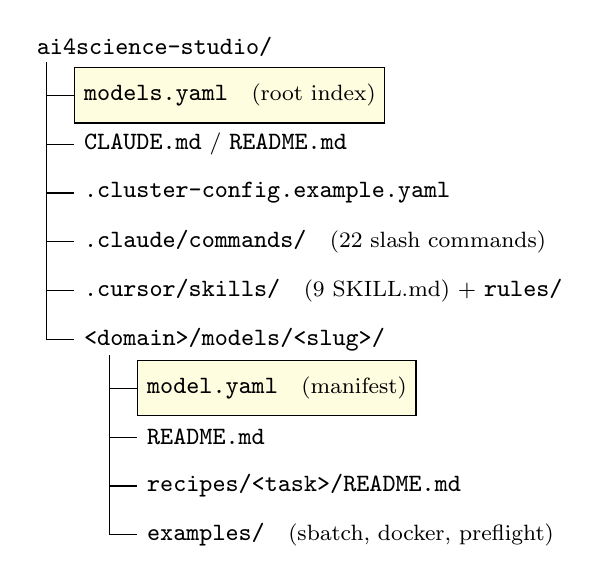
\begin{tikzpicture}[
  every node/.style={font=\footnotesize,anchor=west},
  root/.style={font=\footnotesize\bfseries},
  xshift=0pt,
]
\def\rowsep{0.62}
\node[root] (root) at (0,0) {\file{ai4science-studio/}};
\node[file] (mi)  at (0.6,-1*\rowsep) {\file{models.yaml}\quad(root index)};
\node       (cl)  at (0.6,-2*\rowsep) {\file{CLAUDE.md} / \file{README.md}};
\node       (cc)  at (0.6,-3*\rowsep) {\file{.cluster-config.example.yaml}};
\node       (cmd) at (0.6,-4*\rowsep) {\file{.claude/commands/}\quad(22 slash commands)};
\node       (sk)  at (0.6,-5*\rowsep) {\file{.cursor/skills/}\quad(9 SKILL.md) + \file{rules/}};
\node       (dom) at (0.6,-6*\rowsep) {\file{<domain>/models/<slug>/}};
\node[file] (my)  at (1.4,-7*\rowsep) {\file{model.yaml}\quad(manifest)};
\node       (rm)  at (1.4,-8*\rowsep) {\file{README.md}};
\node       (rec) at (1.4,-9*\rowsep) {\file{recipes/<task>/README.md}};
\node       (ex)  at (1.4,-10*\rowsep) {\file{examples/}\quad(sbatch, docker, preflight)};

\foreach \n in {mi,cl,cc,cmd,sk,dom} {
  \draw (0.25,-0.2) |- (\n.west);
}
\foreach \n in {my,rm,rec,ex} {
  \draw (1.05,{-6*\rowsep-0.2}) |- (\n.west);
}
\end{tikzpicture}
\caption{Repository directory hierarchy. The two entry points for an agent are
\file{models.yaml} (discovery) and each model's \file{model.yaml} (execution
parameters). Domain values are \code{earth\_science}, \code{material\_science},
\code{healthcare}, \code{physics\_simulation}, and \code{protein\_folding}.}
\label{fig:tree}
\end{figure}

\subsection{Model Inventory}
The catalog spans sixteen models across five domains, summarized in
\Cref{tab:inventory}. Earth science is the deepest domain; protein folding is
currently empty, for reasons discussed in \Cref{sec:domains}.

\begin{longtable}{@{}p{2.7cm}p{2.5cm}p{3.2cm}p{3.6cm}@{}}
\caption{Model inventory. HF id \code{N/A} indicates weights hosted outside the
Hugging Face Hub (e.g.\ Google Cloud Storage or GitHub releases).}
\label{tab:inventory}\\
\toprule
\textbf{Model} & \textbf{Domain} & \textbf{License} & \textbf{Primary task} \\
\midrule
\endfirsthead
\toprule
\textbf{Model} & \textbf{Domain} & \textbf{License} & \textbf{Primary task} \\
\midrule
\endhead
\bottomrule
\endfoot
StormCast     & earth science    & Apache-2.0            & Convection-allowing emulation \\
ORBIT-2       & earth science    & See model card        & Downscaling (vision FM) \\
ArchesWeather & earth science    & See model card        & Global forecast + training \\
Aurora        & earth science    & CC-BY-NC-SA-4.0       & Earth-system foundation model \\
GenCast       & earth science    & CC-BY-NC-SA-4.0       & Diffusion ensemble forecast \\
NeuralGCM     & earth science    & Apache-2.0 / CC-BY-SA & Hybrid physics-ML GCM \\
PanguWeather  & earth science    & CC-BY-NC-SA-4.0       & Global forecast (3D nets) \\
MatterGen     & material science & MIT                   & Generative materials design \\
HydraGNN      & material science & BSD-3-Clause-Clear    & Atomistic graph FM \\
GP-MoLFormer  & healthcare       & Apache-2.0            & Molecule generation \\
SwinUNETR     & healthcare       & Apache-2.0            & 3D medical segmentation \\
SemlaFlow     & healthcare       & MIT                   & 3D molecular generation \\
REINVENT4     & healthcare       & Apache-2.0            & RL molecular design \\
MATEY         & physics sim.     & MIT                   & Spatiotemporal surrogate \\
Walrus        & physics sim.     & MIT                   & Continuum dynamics FM \\
\end{longtable}

\subsection{The Agent-First Interface}
An AI coding agent reads \file{models.yaml} to enumerate available models, opens
the target \file{model.yaml} for execution parameters, consults the domain
\file{SKILL.md} for validated patterns, and invokes an appropriate \code{/run-<model>}
slash command. A human, by contrast, reads a per-model \file{README.md} and runs
\file{docker\_run.sh} manually. Both paths converge on the same scripts; the agent
path adds discovery and configuration automation.

\subsection{Studio Web Application}
An optional web application (\file{studio/}) wraps the same YAML tree. Its FastAPI
backend reads the manifests, builds SLURM submission wrappers that delegate to each
model's \file{examples/} scripts, polls job state, and streams logs over
server-sent events. A React/Vite frontend presents a five-step wizard (domain,
model, configure, run, analyze). The backend supports a \emph{demo} mode that runs
synthetic data generators locally without a GPU, and a \emph{live} mode that submits
to SLURM. As discussed in \Cref{sec:weaknesses}, the backend currently hardcodes a
site-specific shared path, which limits portability.

% ===========================================================================
\section{Container and Runtime Strategy}
\label{sec:container}
% ===========================================================================

This section is the most technically detailed, as the container strategy is both
the system's most significant engineering contribution and the source of its most
acute operational friction.

\subsection{Dual-Runtime Design}
Every model ships two launch paths. The first is an Apptainer~\cite{apptainer2021,
kurtzer2017singularity} SLURM script (\file{sbatch\_<task>\_amd.sh}) that runs the
model under \code{srun --mpi=pmix} with the \code{--rocm} flag for GPU passthrough.
The second is a Docker script (\file{docker\_run.sh}) that auto-detects whether an
AMD Container Toolkit runtime is present or whether device files
(\code{/dev/kfd}, \code{/dev/dri/renderD*}) must be passed through directly. Both
paths use the same ROCm/PyTorch base image.

The rationale is sound: Apptainer is the de facto standard in multi-user HPC
because it runs unprivileged and integrates with the batch scheduler, whereas
Docker is more convenient for single-node developer workflows. Maintaining both
doubles the script surface but serves genuinely different environments.

\subsection{The Overlay Strategy}
ROCm/PyTorch SIF images ship a pre-built virtual environment at \code{/opt/venv}
containing a ROCm-compiled PyTorch. Upstream models add heavy dependencies
(\code{earth2studio}, \code{pytorch-lightning}, \code{xformers}) that must be
installed on top. A naive \code{pip install --target} into a bind-mounted directory
resolves packages from scratch and, because packages like \code{earth2studio}
declare \code{torch} as a transitive dependency, pip downloads a fresh multi-GB
CUDA-tagged torch wheel that both wastes space and shadows the correct ROCm build.

The system's answer is a persistent ext3 \emph{overlay} image. Packages are
installed into a staging area, the CUDA \code{torch}/\code{nvidia}/\code{triton}
trees are stripped, and the remainder is copied into the overlay, which future
jobs mount read-only. \Cref{fig:overlay} depicts the pipeline and the failure
points encountered in practice.

\begin{figure}[ht]
\centering
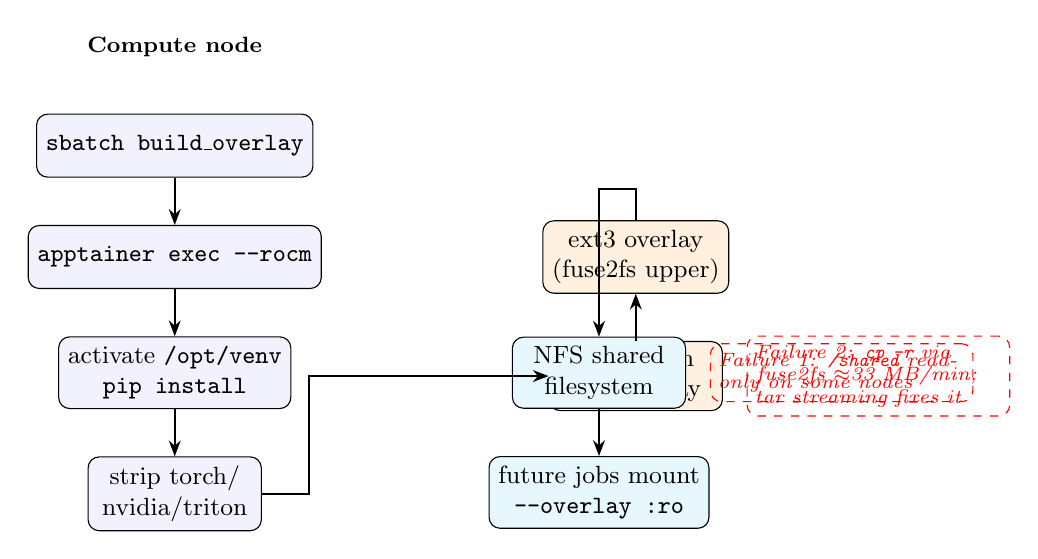
\begin{tikzpicture}[node distance=6mm and 10mm]
% lanes labels
\node[font=\bfseries\footnotesize] (l1) {Compute node};
\node[block,below=of l1] (submit) {\code{sbatch build\_overlay}};
\node[block,below=of submit] (exec) {\code{apptainer exec --rocm}};
\node[block,below=of exec] (pip) {activate \code{/opt/venv}\\\code{pip install}};
\node[block,below=of pip] (strip) {strip torch/\\nvidia/triton};

\node[block,right=28mm of exec,fill=orange!12] (ext3) {ext3 overlay\\(fuse2fs upper)};
\node[block,below=of ext3,fill=orange!12] (tarpack) {tar stream\\into overlay};

\node[block,right=28mm of pip,fill=cyan!10] (nfs) {NFS shared\\filesystem};
\node[block,below=of nfs,fill=cyan!10] (reuse) {future jobs mount\\\code{--overlay :ro}};

\draw[arrow] (submit) -- (exec);
\draw[arrow] (exec) -- (pip);
\draw[arrow] (pip) -- (strip);
\draw[arrow] (strip.east) -- ++(0.6,0) |- (tarpack.west);
\draw[arrow] (tarpack) -- (ext3);
\draw[arrow] (ext3.north) -- ++(0,0.4) -| (nfs.north);
\draw[arrow] (nfs) -- (reuse);

% failure annotations
\node[draw,red,dashed,rounded corners,font=\scriptsize\itshape,right=3mm of nfs,text width=3.1cm]
  {Failure 1: \code{/shared} read-only on some nodes};
\node[draw,red,dashed,rounded corners,font=\scriptsize\itshape,right=3mm of tarpack,text width=3.1cm]
  {Failure 2: \code{cp -r} via fuse2fs $\approx$33 MB/min; tar streaming fixes it};
\end{tikzpicture}
\caption{Overlay build pipeline. Packages are installed into the SIF venv, the CUDA
trees are stripped, and the result is streamed into an ext3 overlay that is copied to
NFS for reuse. Two operational failure modes discovered during the StormCast build are
annotated.}
\label{fig:overlay}
\end{figure}

\begin{weakness}{Overlay build fragility}
The StormCast overlay required four attempts before succeeding. The first two failed
because \code{/shared} was mounted read-only on the assigned compute node, a condition
not detectable before job submission. A third attempt reached the copy stage but
\code{cp -r} into the ext3 overlay via \code{fuse2fs} achieved only about 33~MB/min,
so 1.5~GB of many small files did not finish within the wall-clock limit. The final,
successful build replaced \code{cp -r} with \code{tar} streaming and split the work
into a stage job and an overlay-assembly job. The tradeoff (build complexity for
fast job startup) is defensible, but the failure modes are opaque and no
pre-submission check exists to catch them.
\end{weakness}

\subsection{ROCm Userspace and Host Driver Compatibility}
A recurring hazard is silent CPU fallback: \code{torch.cuda.is\_available()} returns
false even when GPU devices are visible inside the container, caused by a mismatch
between the container's ROCm userspace and the host's kernel driver. The skill files
record a validated pairing (a ROCm~7.0 image fails against a particular host driver,
while the ROCm~7.2.2 image works) and document \code{HSA\_OVERRIDE\_GFX\_VERSION} as a
workaround for architecture-string mismatches. Capturing this in a queryable form is
valuable because the failure is silent and easily misattributed to model code.

\subsection{Canonical Image Strategy}
All recently added models converge on a single base image,
\code{rocm/pytorch:rocm7.2.2\_ubuntu24.04\_py3.12\_pytorch\_release\_2.10.0}. The same
image covers MI250X (gfx90a), MI300X (gfx942), and MI350X (gfx950), differentiated
only by a wheel-tag parameter and, where needed, an architecture override. This is a
strong decision: one image, parameter-driven architecture selection, minimizes the
matrix of things that can break.

\begin{strength}{Single parameterized base image}
Converging on one ROCm/PyTorch image across three GPU generations reduces the
maintenance surface dramatically. Architecture selection is a parameter, not a
separate image, so a new GPU generation is onboarded by updating one tag rather than
forking the recipe set.
\end{strength}

\subsection{Common HPC Patterns Captured}
The skill files codify hard-won patterns: never clobbering inherited environment
variables (always append with \code{\$\{VAR:-\}}); resolving the script directory via
\code{scontrol} to avoid the SLURM spool; using \code{--mpi=pmix} for multi-rank
Apptainer jobs; probing GPU health with a one-line Python check before the main run;
and avoiding an \code{MPI\_Init} collision when wrapping a pmix \code{srun} inside a
\code{python3 -c} scaffold. \Cref{tab:isolation} compares the overlay approach to
alternative isolation strategies.

\begin{table}[ht]
\centering
\footnotesize
\caption{Dependency-isolation strategies compared.}
\label{tab:isolation}
\begin{tabular}{@{}p{3.1cm}p{2.0cm}p{2.0cm}p{2.0cm}p{3.0cm}@{}}
\toprule
\textbf{Strategy} & \textbf{Per-job overhead} & \textbf{Reproducibility} & \textbf{Space} & \textbf{Notes} \\
\midrule
Apptainer ext3 overlay & Low (build once) & Medium (no hashing) & Good (1.7--7 GB) & HPC-native; build fragile \\
venv in container & Medium & Medium & Good & Rebuild per job or bind-mount \\
Conda environment & High (solver) & Low & Poor & Often unavailable without module \\
\code{pip --target} bind & Low--Medium & Low & Good & Ad hoc; implicit deps \\
Full fat SIF & Zero per job & High (immutable) & Poor (multi-GB) & Rebuild SIF for any change \\
\bottomrule
\end{tabular}
\end{table}

% ===========================================================================
\section{Agent-First Design Pattern}
\label{sec:agent}
% ===========================================================================

\subsection{Metadata-Driven Execution}
The two-layer metadata design separates discovery (\file{models.yaml}) from
execution (\file{model.yaml}). Because execution parameters live in data rather
than in agent instructions, the agent needs no hardcoded knowledge of any specific
model; it can enumerate, compare, and launch models purely by reading manifests.
This resembles the model-card convention popularized by the Hugging Face
Hub~\cite{lhoest2021huggingface,wolf2020huggingface}, extended with HPC-specific
fields (container image, environment variables, validated hardware).

\subsection{Slash Commands and Skills}
Twenty-two slash commands in \file{.claude/commands/} encode runnable workflows
(discovery, auditing, adding models, and per-model \code{/run-*} launchers). Nine
skill files in \file{.cursor/skills/} inject validated context during the agent's
planning phase. The distinction matters: commands are executable procedures, skills
are reference knowledge. Together they form agent-facing infrastructure rather than
human documentation.

\subsection{Organic Lesson Propagation}
A distinctive rule (\file{cross-model-lesson-reuse.mdc}) requires that every fix
propagate to sibling models sharing the pattern, to the cross-runtime equivalent
(Apptainer $\leftrightarrow$ Docker), and into the relevant skill file. The
governing heuristic is a litmus test: \emph{would a fresh agent session make the
same mistake?} If yes, the fix is incomplete.

\begin{strength}{Session-durable institutional memory}
In a codebase maintained largely by AI agents, institutional knowledge is by default
session-scoped and lost between conversations. The skill files act as durable working
memory that a fresh agent reads before acting, and the propagation rule keeps that
memory consistent across models and runtimes. This is a thoughtful answer to a real
problem in agent-maintained repositories.
\end{strength}

\subsection{Multi-Agent Performance Analysis}
The performance-analysis workflow (\Cref{fig:perfdag}) orchestrates specialized
subagents. A launcher submits the job and records a manifest; analyst pairs then read
a PyTorch trace (TraceLens) and a time-series metrics store (Omnistat) in parallel;
verifier pairs independently re-derive each analyst claim; and a synthesizer combines
only the surviving claims. Refuted claims remain in the report marked as refuted. A
machine-readable \file{lever\_catalog.yaml} tracks every optimization attempt with a
risk rating, expected payoff, revert method, and evidence citation.

\begin{figure}[ht]
\centering
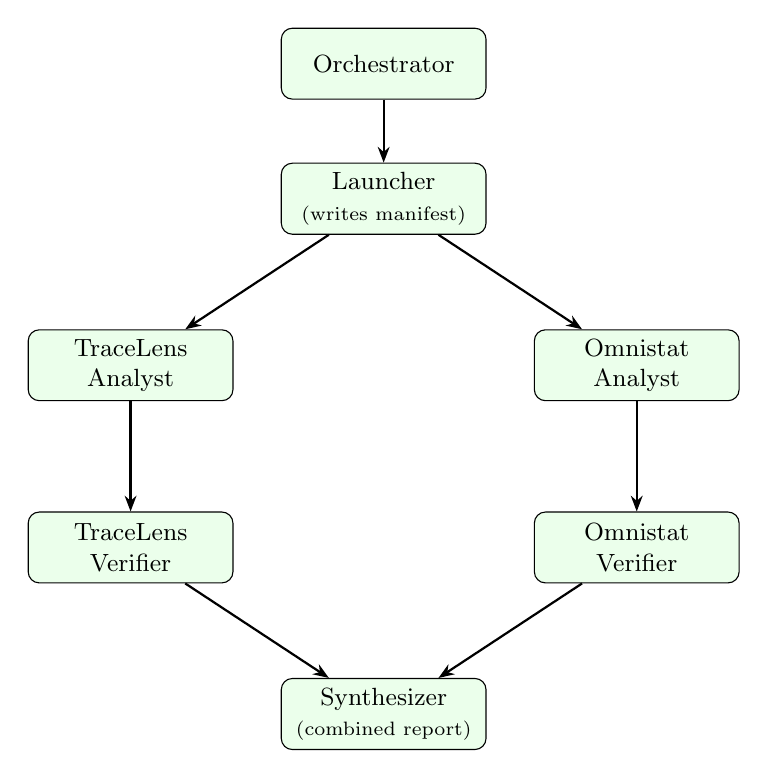
\begin{tikzpicture}[node distance=8mm and 14mm]
\node[agent] (orch) {Orchestrator};
\node[agent,below=of orch] (launch) {Launcher\\\scriptsize(writes manifest)};
\node[agent,below left=12mm and 6mm of launch] (ta) {TraceLens\\Analyst};
\node[agent,below right=12mm and 6mm of launch] (oa) {Omnistat\\Analyst};
\node[agent,below=14mm of ta] (tv) {TraceLens\\Verifier};
\node[agent,below=14mm of oa] (ov) {Omnistat\\Verifier};
\node[agent,below right=12mm and 6mm of tv] (syn) {Synthesizer\\\scriptsize(combined report)};

\draw[arrow] (orch) -- (launch);
\draw[arrow] (launch) -- (ta);
\draw[arrow] (launch) -- (oa);
\draw[arrow] (ta) -- (tv);
\draw[arrow] (oa) -- (ov);
\draw[arrow] (tv) -- (syn);
\draw[arrow] (ov) -- (syn);
\end{tikzpicture}
\caption{Multi-agent performance-analysis workflow. Analyst claims must survive
independent re-derivation by a verifier before the synthesizer accepts them; refuted
claims are retained and labeled. Each edge carries a defined input/output contract
(manifest, trace files, \file{verified\_claims.json}).}
\label{fig:perfdag}
\end{figure}

\begin{strength}{Adversarial verification of performance claims}
Requiring an independent verifier to confirm or refute each analyst finding, and
retaining refuted claims in the report, is a rigorous practice rarely seen in HPC
performance tooling. Combined with the \file{lever\_catalog.yaml} audit trail, it
brings a measure of reproducibility to performance-optimization work.
\end{strength}

\subsection{Limitations of the Agent-First Approach}
The design excels at discovery and at executing well-defined workflows, but it is
weaker for novel configurations. The \file{.cluster-config.yaml} mechanism is sound
in principle, yet several scripts retain hardcoded site fallbacks that override it
(\Cref{sec:weaknesses}). Agent behavior is also non-deterministic and dependent on an
external LLM service, so reproducing a past run is harder than re-invoking a versioned
API. Finally, the main skill file is large enough that injecting it wholesale competes
with task context for the agent's token budget.

% ===========================================================================
\section{Domain Coverage Analysis}
\label{sec:domains}
% ===========================================================================

\subsection{Earth Science (seven models)}
This is the strongest domain, spanning deterministic global forecasting
(PanguWeather~\cite{bi2023panguweather}, Aurora~\cite{bodnar2025aurora}),
diffusion-based ensembles (GenCast~\cite{price2025gencast}), convection-allowing
high resolution (StormCast~\cite{bodnar2024stormcast}), downscaling
(ORBIT-2~\cite{wang2025orbit2}), hybrid physics-ML general circulation
(NeuralGCM~\cite{kochkov2023neuralgcm}), and a training-capable model
(ArchesWeather~\cite{couairon2024archesweather}). Several models carry a data
barrier: staged ERA5 in zarr, credentials for the Copernicus data store, or
full-node HBM for the highest resolutions.

\subsection{Material Science (two models)}
HydraGNN~\cite{lupopasini2024hydragnn} is a graph foundation model with full
training, inference, and a performance-optimization loop; MatterGen~\cite{zeni2025mattergen}
is a diffusion-based generative model for inorganic materials. The domain is thin in
count but deep in recipe quality for HydraGNN.

\subsection{Healthcare and Life Sciences (four models)}
GP-MoLFormer~\cite{ross2023gpmolformer} (molecule generation),
SwinUNETR~\cite{hatamizadeh2022swinunetr} (3D medical segmentation, built on the
Swin Transformer~\cite{liu2021swin}), SemlaFlow~\cite{morehead2024semlaflow} (3D
molecular generation), and REINVENT4~\cite{loeffler2024reinvent4} (RL molecular
design). A mandatory research-only disclaimer and a prohibition on
patient-identifiable data are enforced by a domain rule.

\subsection{Physics Simulation (two models)}
MATEY~\cite{subramanian2024matey} (spatiotemporal surrogate) and
Walrus~\cite{mccabe2025walrus} (cross-domain continuum-dynamics foundation model).
Coverage is thin but the direction is promising.

\subsection{Protein Folding (zero models)}
The domain directory exists but registers no models. AlphaFold~3's model-parameter
license restricts redistribution and limits permitted uses~\cite{abramson2024alphafold3},
which likely explains the absence of a redistributable recipe. This is a clear
opportunity: ESMFold~\cite{lin2023esmfold} is MIT-licensed and Hugging Face-hosted,
making it the natural first entry.

% ===========================================================================
\section{Case Study: The ADIOS2 Dependency}
\label{sec:adios}
% ===========================================================================

HydraGNN is the only model in the catalog that depends on
ADIOS2~\cite{godoy2020adios2}, and its build is the most complex in the repository.
We examine it in detail because it is both instructive and a concrete simplification
target.

\subsection{Why ADIOS2 Is Used}
HydraGNN trains on more than 154 million atomistic structures, delivered as
pre-processed BP4-format datasets (for example ANI1x at 30~GB and Alexandria at
23~GB). Its data loader, \code{AdiosMultiDataset}, uses ADIOS2 for MPI-collective
parallel I/O: each rank opens the \code{.bp} datasets directly, dataset metadata is
broadcast once at startup over the management network, and the training hot path
carries no central I/O bottleneck. This design targets the multi-node,
many-GPU regime for which ADIOS2 was built.

\subsection{Install Complexity}
Unlike the other dependencies, ADIOS2 has no binary wheel on PyPI, so the overlay
build compiles it from source with CMake inside the container, configured with
\code{ADIOS2\_USE\_MPI=ON} against the host OpenMPI. The build additionally requires
\code{cmake}, \code{nanobind}, and \code{mpi4py}. On an HPC node the compile is fast
(the full overlay build, ADIOS2 included, completes in roughly three and a half
minutes), but the resulting shared libraries are linked against the exact host MPI,
so \code{LD\_LIBRARY\_PATH} must expose both the ADIOS2 libraries and the OpenMPI
libraries at run time.

\begin{lesson}{ADIOS2 re-mmap at epoch boundaries}
Without \code{persistent\_workers=True}, PyTorch forks fresh DataLoader workers at
every epoch, and each worker re-imports the dataset module and re-mmaps the ADIOS2
BP files. This produces a bimodal iteration-time distribution with a long tail at
epoch boundaries. A local patch sets \code{persistent\_workers=True} when
\code{num\_workers > 0}, eliminating the re-mmap overhead. This is a strong
candidate for an upstream contribution.
\end{lesson}

\subsection{Inference Does Not Need ADIOS Data}
Inference reads only a checkpoint and a JSON config through standard PyTorch and
JSON I/O; it never touches an ADIOS dataset. However, \code{import hydragnn}
transitively imports the ADIOS dataset module at load time, so the \code{adios2}
package must at least be importable even for inference. This is the crux of the
simplification opportunity.

\subsection{ADIOS2 Versus Alternatives}
\Cref{tab:adios} compares ADIOS2 to common alternatives. ADIOS2 is justified at
multi-node scale but heavy for single-node inference or small fine-tuning datasets.

\begin{table}[ht]
\centering
\footnotesize
\caption{Data-format options for HydraGNN-style atomistic graph data.}
\label{tab:adios}
\begin{tabular}{@{}p{3.4cm}p{2.4cm}p{2.6cm}p{2.4cm}p{2.6cm}@{}}
\toprule
\textbf{Approach} & \textbf{Parallel I/O} & \textbf{Install} & \textbf{HPC maturity} & \textbf{Interoperability} \\
\midrule
ADIOS2 BP4 (current) & Yes (MPI-native) & High (CMake+MPI) & High & Low (specialized) \\
HDF5 / h5py & Yes (PHDF5) & Low (wheel) & High & High \\
Zarr + fsspec & Yes (chunked) & Low (pip) & Medium & High \\
numpy \code{.npz} & No & Zero & Low & High \\
PyG InMemoryDataset & No & Low (PyG) & Low & High \\
\bottomrule
\end{tabular}
\end{table}

\subsection{Simplification Paths}
Four options, roughly in increasing order of effort:
\begin{enumerate}
  \item \textbf{Inference-only overlay without MPI ADIOS.} Build a lightweight overlay
    that omits \code{ADIOS2\_USE\_MPI=ON}; a non-MPI \code{adios2} satisfies the import
    without the CMake-plus-MPI build. Only the training overlay needs the full build.
  \item \textbf{Guard the import.} A small upstream change wrapping the ADIOS import in
    a try/except (or gating it behind a mode flag) removes the dependency for inference
    users entirely.
  \item \textbf{HDF5 for small datasets.} For fine-tuning data under roughly 10~GB,
    HDF5 via h5py is far simpler to install and broadly supported; ADIOS2 only becomes
    necessary at large multi-node scale.
  \item \textbf{DDStore for 32+ nodes.} At very large scale, per-rank ADIOS I/O itself
    becomes the bottleneck and the upstream DDStore aggregation path is the intended
    solution; it is currently noted as future work.
\end{enumerate}

% ===========================================================================
\section{Identified Architectural Weaknesses}
\label{sec:weaknesses}
% ===========================================================================

\subsection{Site-Specific Hardcoding}
The repository as cloned is not directly usable at a second HPC site without editing
several files. The root-level \file{build\_*.slurm} scripts embed a specific
partition, account, and absolute home-directory paths. The Studio backend
(\file{studio/backend/jobs.py}) hardcodes a shared-directory prefix and per-model
overlay paths rather than reading \file{.cluster-config.yaml}, even though a
well-structured \file{.cluster-config.example.yaml} exists.

\begin{weakness}{Config exists but is not wired in}
The gap between the configuration system's design intent and its actual use is the
single most impactful portability risk. The schema for site configuration is already
defined; the backend and the root build scripts simply do not consume it. Closing this
gap is low effort and high value (\Cref{sec:recommendations}, items 1--2).
\end{weakness}

\subsection{Overlay Build Fragility}
Documented in \Cref{sec:container} and \Cref{fig:overlay}: read-only \code{/shared} on
some nodes, poor \code{fuse2fs} throughput for many small files, and the absence of a
pre-submission precondition check. The tar-streaming, two-job pattern that finally
succeeded should be promoted from an ad hoc fix to the default build recipe.

\subsection{No Functional Validation or CI}
The only automated check is a weekly CodeQL security scan for Python. There is no
schema validation for manifests, no syntax check for scripts, and no smoke test that a
newly added model can be launched. The organic-propagation discipline is enforced by
agents, not by machines, so a regression can enter the repository undetected.

\subsection{Skill-File Monolith}
The main skill file has grown large enough that injecting it wholesale consumes a
meaningful share of an agent's context budget. Domain-specific skill files mitigate
this only partially, because cross-cutting lessons still accumulate centrally.
Topic-based segmentation would reduce token pressure.

\subsection{No Model-Weight Version Pinning}
No manifest records a weight revision or checksum. Hugging Face repositories can change
default branches, rename shards, or add files, and non-HF weights on cloud buckets are
even less stable. Recipes can therefore break silently when upstream artifacts move.

\subsection{Committed Synthetic and Demo Artifacts}
Several synthetic fine-tuning datasets are committed under \file{studio/synthetic\_data/},
and demo output lives under the Studio tree. Although synthetic, their presence conflates
a code repository with a data repository and will grow if regenerated. They are not
excluded by \file{.gitignore}.

\subsection{Documentation Gap}
The \file{docs/} directory currently contains only images. The content that would serve
as administrator-facing documentation is scattered across \file{CLAUDE.md}, the skill
files (written for agents), and per-model READMEs. There is no single
``deploy this at a new HPC site'' guide. (This review is a first step toward closing
that gap.)

% ===========================================================================
\section{Strengths in Depth}
\label{sec:strengths}
% ===========================================================================

\subsection{Near-Zero Installation Friction}
\code{git clone} plus a handful of environment variables is the onboarding path. No
package manager, no compilation, and no dependency resolution at the repository level.
For an HPC user this is a real advantage over framework-based alternatives that require
a pip install and a solver step. The dual-runtime scripts with auto-detection extend
this portability across clusters and laptops.

\subsection{Consistent Metadata Catalog}
A uniform manifest schema across all sixteen models enables programmatic discovery,
comparison, and a single-pass readiness audit. This consistency is what makes the
agent-first interface tractable.

\subsection{Living Knowledge Base}
The skill files capture validated, otherwise-undocumented AMD/ROCm workarounds:
attention-kernel batch-grid limits, MIOpen configuration inherited from production
practice, memory-format dead ends, and multi-node partitioning rules. Rediscovering
these would cost substantial effort; capturing them in a queryable form is a genuine
asset.

\subsection{Systematic Performance Methodology}
The analyst/verifier/synthesizer workflow and the lever catalog (\Cref{sec:agent})
apply reproducible-research practices to HPC performance work, a combination rarely
found in model-collection repositories.

% ===========================================================================
\section{Competitive Landscape}
\label{sec:competition}
% ===========================================================================

\Cref{tab:competition} positions AI4Science Studio against representative
alternatives. The comparison axes are hardware focus, installation path, HPC
nativity, testing maturity, agent integration, and catalog size.

\begin{table}[ht]
\centering
\footnotesize
\caption{Competitive comparison. ``HPC native'' means designed for unprivileged
multi-user batch execution (Apptainer/SLURM). Model counts are approximate.}
\label{tab:competition}
\begin{tabular}{@{}p{3.0cm}p{1.9cm}p{1.7cm}p{1.2cm}p{1.5cm}p{1.5cm}@{}}
\toprule
\textbf{System} & \textbf{Hardware} & \textbf{Install} & \textbf{HPC native} & \textbf{Testing} & \textbf{Agent UI} \\
\midrule
AI4Science Studio & AMD Instinct & git clone & Yes & CodeQL only & Yes \\
BioNeMo~\cite{bionemo2024} & NVIDIA & pip / NGC & Partial & Full CI & No \\
earth2studio~\cite{earth2studio2024} & NVIDIA & pip & No & CI & No \\
HF Transformers~\cite{wolf2020huggingface} & Any & pip & Partial & Full CI & Via API \\
LUMI-AI recipes~\cite{lumiairecipes} & AMD/NVIDIA & git clone & Yes & Minimal & No \\
FAIR-Chem~\cite{fairchem2024} & NVIDIA & pip & Partial & Full CI & No \\
AlgoPerf~\cite{dahl2023algoperf} & Any & pip & Partial & Yes & No \\
\bottomrule
\end{tabular}
\end{table}

AI4Science Studio occupies a distinctive niche: it is the only system in the
comparison explicitly designed for agent-mediated interaction, and the only one
targeting AMD Instinct under Apptainer and SLURM as a first-class case. Relative to
pip-installable frameworks it lacks a Python API, versioned releases, and CI. Relative
to other recipe collections such as the LUMI-AI scripts, it offers a considerably more
sophisticated agent interface and richer HPC pattern documentation, at the cost of
being tightly coupled to AMD ROCm.

% ===========================================================================
\section{Architectural Decision Analysis}
\label{sec:decisions}
% ===========================================================================

\subsection{Overlay Versus venv Versus Conda}
Summarized in \Cref{tab:isolation}. The overlay trades a fragile, occasionally slow
build for fast, immutable job startup. For a site that builds once and runs many jobs,
the tradeoff is reasonable, provided the build is made robust (\Cref{sec:recommendations}).

\subsection{Agent-First Versus Framework-First}
An agent-first system is more flexible and requires no installation, but is harder to
test and depends on a non-deterministic external service. A framework-first system
offers type checking, IDE support, and testability at the cost of installation and
dependency management. AI4Science Studio is firmly agent-first; adding a thin,
testable Python or shell layer for the most common operations would capture some
framework-first benefits without abandoning the model.

\subsection{YAML Manifest Versus Python API}
YAML manifests are readable by agents, shell scripts, the web app, and humans, which
is precisely what enables the multi-consumer architecture. The cost is that there is no
importable API and no compile-time checking of the manifests. A lightweight schema
validator would recover much of the safety without sacrificing accessibility.

\subsection{Link Versus Vendor}
Keeping upstream code and weights external keeps the repository small but couples every
recipe to upstream availability and API stability. When an upstream repository is
restructured or a model card changes its file layout, recipes can break silently. Weight
version pinning (\Cref{sec:recommendations}, item 6) is the main mitigation.

% ===========================================================================
\section{Recommendations}
\label{sec:recommendations}
% ===========================================================================

Recommendations are prioritized by impact against effort. \Cref{tab:recs} summarizes;
the highest-priority items are elaborated below.

\begin{table}[ht]
\centering
\footnotesize
\caption{Prioritized recommendations.}
\label{tab:recs}
\begin{tabular}{@{}clllp{6.4cm}@{}}
\toprule
\textbf{\#} & \textbf{Priority} & \textbf{Effort} & \textbf{Area} & \textbf{Recommendation} \\
\midrule
1  & High   & Low    & Portability & Wire \file{.cluster-config.yaml} into \file{jobs.py} \\
2  & High   & Low    & Portability & Templatize root \file{build\_*.slurm} (no absolute paths) \\
3  & Medium & Medium & Quality     & Per-model smoke tests + CI (schema + CPU preflight) \\
4  & Medium & Medium & Agent UX    & Segment skill files by topic \\
5  & Medium & Medium & Portability & Shared \code{source\_cluster\_config()} for sbatch scripts \\
6  & Medium & Medium & Robustness  & Weight version pinning (\code{weights\_revision}) \\
7  & Medium & Low    & Simplicity  & HydraGNN inference overlay without MPI ADIOS \\
8  & Low    & Low    & Hygiene     & Move synthetic data out of the repo \\
9  & Low    & High   & Coverage    & Add ESMFold to protein folding \\
10 & Low    & Medium & Docs        & Add \file{CLUSTER\_SETUP.md} and \file{ARCHITECTURE.md} \\
11 & Low    & Low    & Robustness  & \code{build\_overlay --dry-run} precondition check \\
12 & Low    & Medium & Upstream    & PR guarded ADIOS import + persistent-workers patch \\
\bottomrule
\end{tabular}
\end{table}

\paragraph{Item 1 (High / Low): Wire the cluster config into the backend.}
Replace the hardcoded shared-directory prefix in \file{jobs.py} with a loader that
reads \file{.cluster-config.yaml} from the repository root, falling back to a
user-level config. The schema already exists; only the reader is missing. This makes
the Studio portable to any site in about a day.

\paragraph{Item 2 (High / Low): Templatize the root build scripts.}
The root \file{build\_*.slurm} files should read partition, account, and paths from the
cluster config or from environment variables with placeholder defaults, and should
contain no absolute home-directory paths. Half a day of work removes the need to hand-edit
these files per site.

\paragraph{Item 3 (Medium / Medium): Add smoke tests and CI.}
A CPU-mode CI job can validate manifest schemas and shell syntax on every push. A
GPU-mode smoke test per model can confirm container launch, GPU visibility, and, where a
synthetic generator exists, a one-step forward pass. This turns the propagation
discipline into a machine-checked guarantee.

\paragraph{Item 7 (Medium / Low): Simplify the HydraGNN build for inference.}
Per \Cref{sec:adios}, an inference-only overlay that omits the MPI ADIOS build removes
the CMake-plus-MPI compile from the most common user path, leaving the full build only
for training.

% ===========================================================================
\section{Conclusion}
\label{sec:conclusion}
% ===========================================================================

AI4Science Studio is a well-conceived agent-first recipe collection that addresses a
real and growing need: running open AI-for-science models on AMD Instinct HPC systems.
Its agent-facing metadata catalog, its durable knowledge base of validated ROCm
workarounds, and its adversarially verified performance methodology are genuine
contributions that distinguish it from both framework-based alternatives and other
recipe collections. Its principal weaknesses, site-specific hardcoding, overlay build
fragility, the absence of functional CI, and an empty protein-folding domain, are all
correctable with modest, well-scoped effort, and the recommendations in
\Cref{sec:recommendations} lay out a concrete path. The system delivers the most value
to sophisticated HPC sites that already operate AMD Instinct hardware and that work with
AI coding agents; it does not aim to provide, and should not be judged against, a
casual \code{pip install} experience.

% ===========================================================================
\appendix
\section{Key File Reference}
\begin{longtable}{@{}p{6.4cm}p{7.2cm}@{}}
\caption{Key files referenced in this review.}\\
\toprule
\textbf{Path} & \textbf{Role} \\
\midrule
\endfirsthead
\toprule
\textbf{Path} & \textbf{Role} \\
\midrule
\endhead
\bottomrule
\endfoot
\file{models.yaml} & Repository-wide model index (agent entry point) \\
\file{<domain>/models/<slug>/model.yaml} & Per-model manifest (execution parameters) \\
\file{.cursor/skills/*/SKILL.md} & Agent knowledge base (validated patterns) \\
\file{.claude/commands/*.md} & Slash commands (runnable workflows) \\
\file{.cursor/rules/*.mdc} & Authoring and propagation rules \\
\file{.cluster-config.example.yaml} & Site configuration schema \\
\file{studio/backend/jobs.py} & Web-app job orchestration (hardcoding to fix) \\
\file{material\_science/models/HydraGNN/examples/build\_overlay\_amd.sh} & ADIOS2 source build \\
\file{build\_stormcast\_*.slurm} & Overlay build jobs (fragility case study) \\
\end{longtable}

\section{Glossary}
\begin{description}
\item[Apptainer / SIF] Unprivileged HPC container runtime; SIF is its single-file image format.
\item[ext3 overlay] A writable filesystem image layered over a read-only SIF at run time.
\item[fuse2fs] The FUSE driver that mounts an ext3 overlay; a throughput bottleneck for many small files.
\item[SLURM / PMIx] HPC batch scheduler and the process-management interface used for multi-rank launch.
\item[RCCL] ROCm Collective Communication Library, the AMD analogue of NCCL for gradient all-reduce.
\item[HBM] High-bandwidth memory on the GPU package.
\item[gfx90a / gfx942 / gfx950] ROCm architecture strings for MI250X, MI300X, and MI350X.
\item[SDPA] Scaled dot-product attention, a fused attention kernel.
\item[FSDP / HSDP] Fully and hybrid sharded data parallelism for large-model training.
\item[ADIOS2] The Adaptable I/O System, an MPI-parallel scientific I/O framework using the BP4 format.
\item[TunableOp] A ROCm feature that auto-selects GEMM implementations at run time.
\end{description}

\bibliographystyle{unsrtnat}
\bibliography{refs/architecture_review}

\end{document}
